\thispagestyle{quantoannone}
\pagestyle{quantoan}
\everymath{\color{quantoan}}
\graphicspath{{../quantoan/pic/}}
\blfootnote{$^1$\color{quantoan}Viện Toán học.}
\begingroup
\AddToShipoutPicture*{\put(0,616){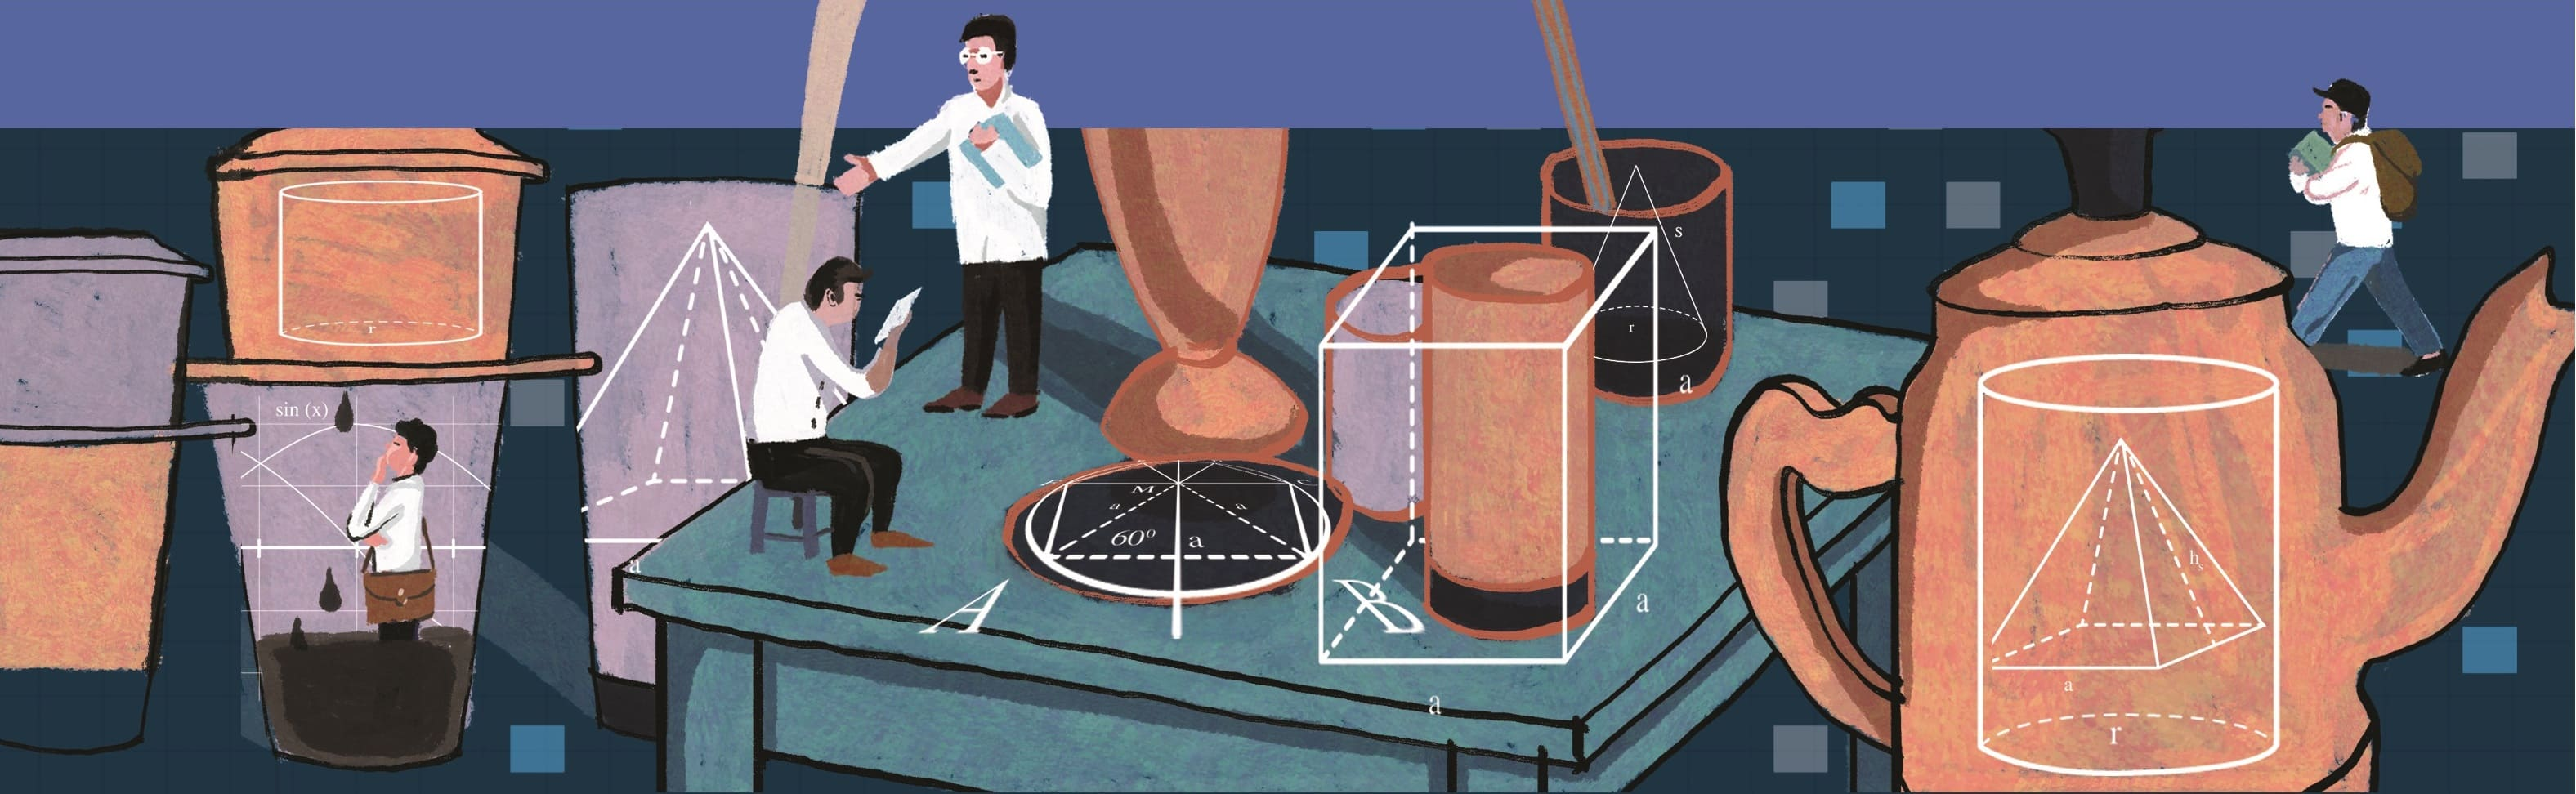
\includegraphics[width=19.3cm]{../bannerquantoan}}}
\AddToShipoutPicture*{\put(118,550){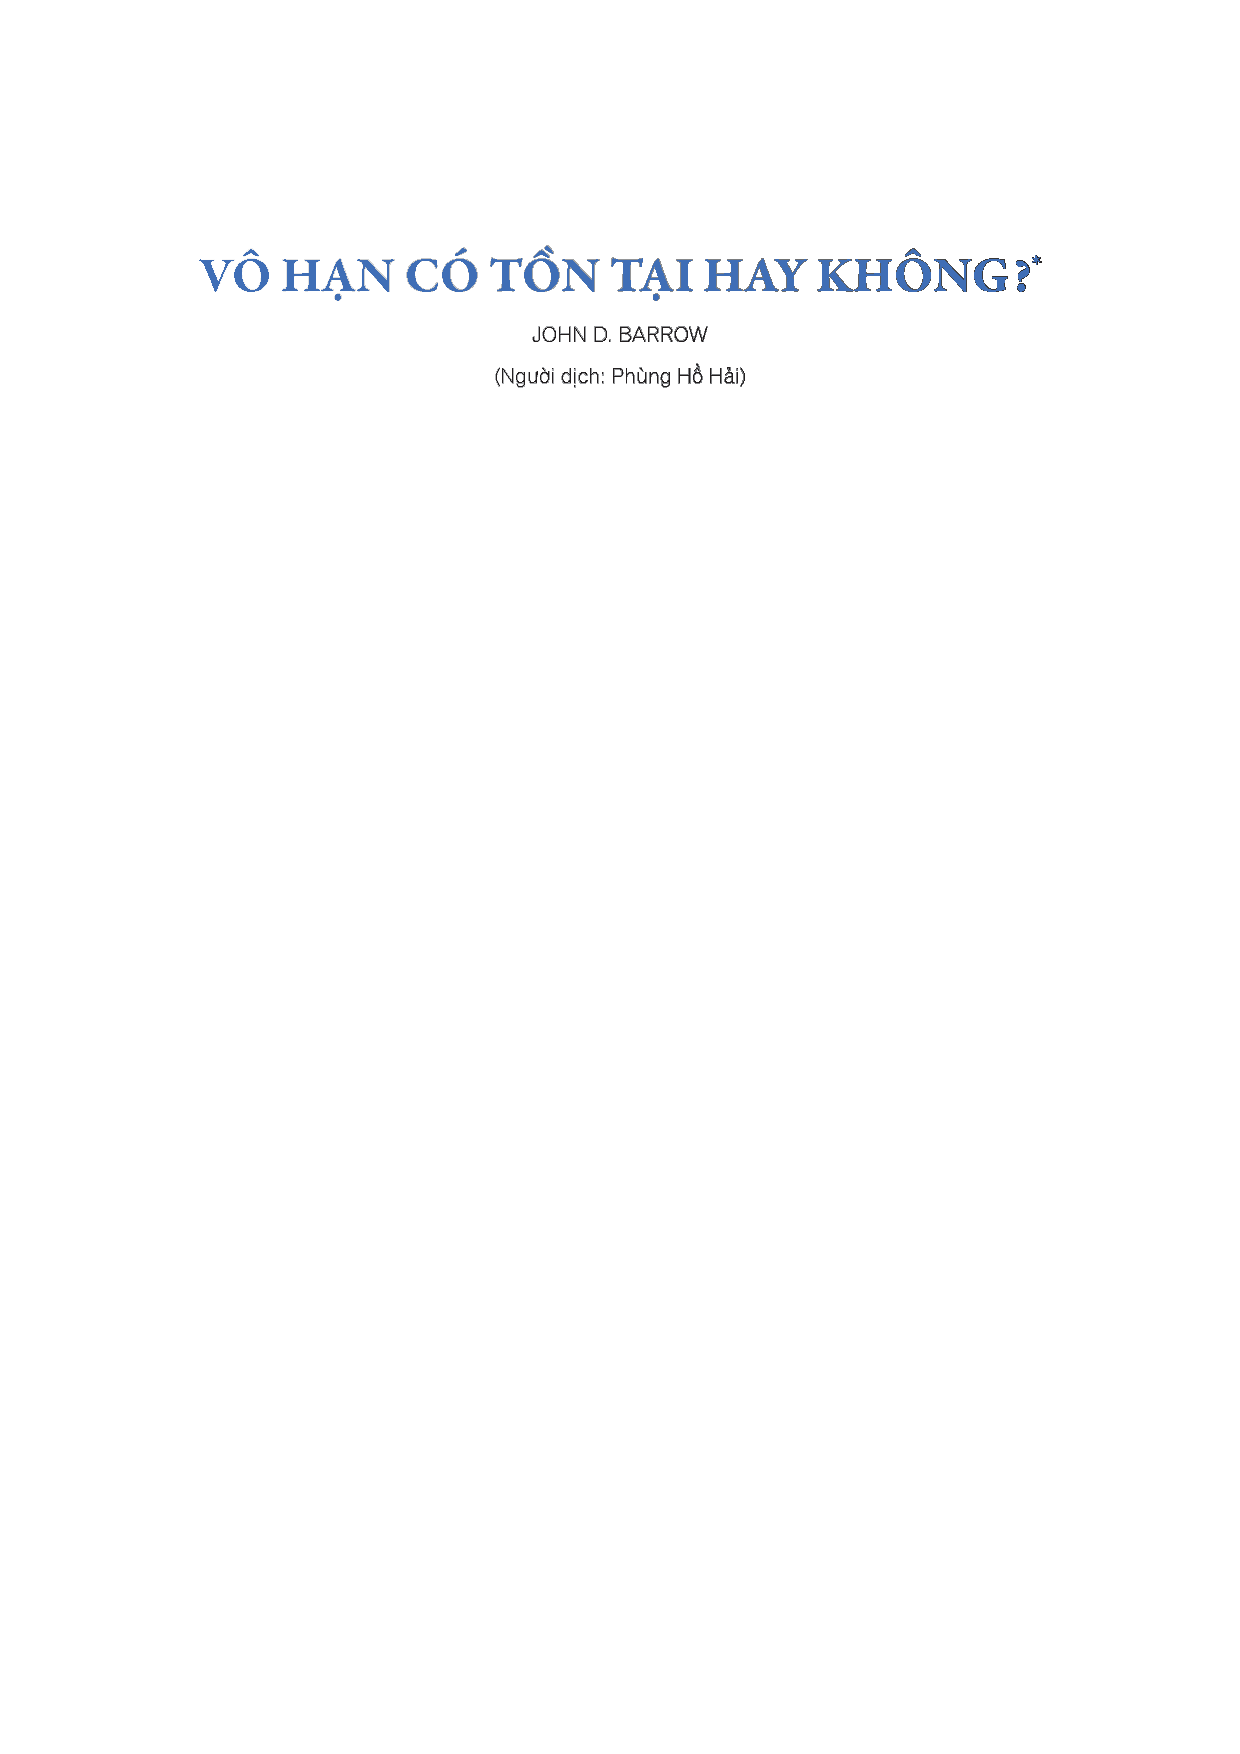
\includegraphics[scale=1]{../tieude1.pdf}}}
\centering
\endgroup

\vspace*{160pt}

\begin{multicols}{2}	
	\textit{Cantor viết: The essence of mathematics lies in its freedom -- Bản chất của toán học nằm ở sự tự do của nó. Cantor là người xây dựng khái niệm tập hợp trong toán học, vẫn đang được sử dụng ngày nay.} 
	\vskip 0.1cm
	Tập hợp được tạo thành từ những phần tử. Tự do của toán học nằm ở chỗ, người ta có thể hình dung phần tử là bất kỳ thứ gì, và tập hợp chúng lại theo bất kỳ cách nào mà người ta muốn. Chẳng hạn có thể coi những chiếc ghế hay những dòng sông là những phần tử và chúng ta có ``tập hợp những chiếc ghế và những dòng sông". 
	\vskip 0.1cm
	Nghe thật vô nghĩa!
	\vskip 0.1cm
	Đúng là vô nghĩa. Rõ ràng chẳng ai rỗi hơi nghĩ ra những điều vô nghĩa. Người ta chỉ tập hợp những phần tử có những liên hệ nào đó lại với nhau, chẳng hạn, tập hợp các chàng trai cùng đang phải lòng một cô gái, hay ngược lại, các cô gái cùng để ý một chàng trai, ... Nói một cách toán học, thì người ta thường xác định tập hợp bằng cách liệt kê hay mô tả các phần tử của nó theo một tính chất nào đó.
	\vskip 0.1cm
	Khi nói về các tập hợp, người ta cũng sẽ nói về những bộ phận của nó. Trong toán học, người ta gọi đó là tập con của một tập hợp. Hoặc là, khi có hai tập hợp, người ta có thể kết hợp chúng lại, hoặc tìm phần chung của chúng, v.v. Đôi khi, hai tập hợp chẳng có gì chung, ta nói giao của chúng bằng \textit{rỗng}. Rỗng cũng được coi là một tập hợp -- một tập hợp ``không có gì". Và, đã là ``không có gì" thì ở đâu cũng thế, cho nên, chỉ có đúng một tập rỗng mà thôi, và nó là tập con của mọi tập hợp! 
	\begin{figure}[H]
		\vspace*{-5pt}
		\centering
		\captionsetup{labelformat= empty, justification=centering}
		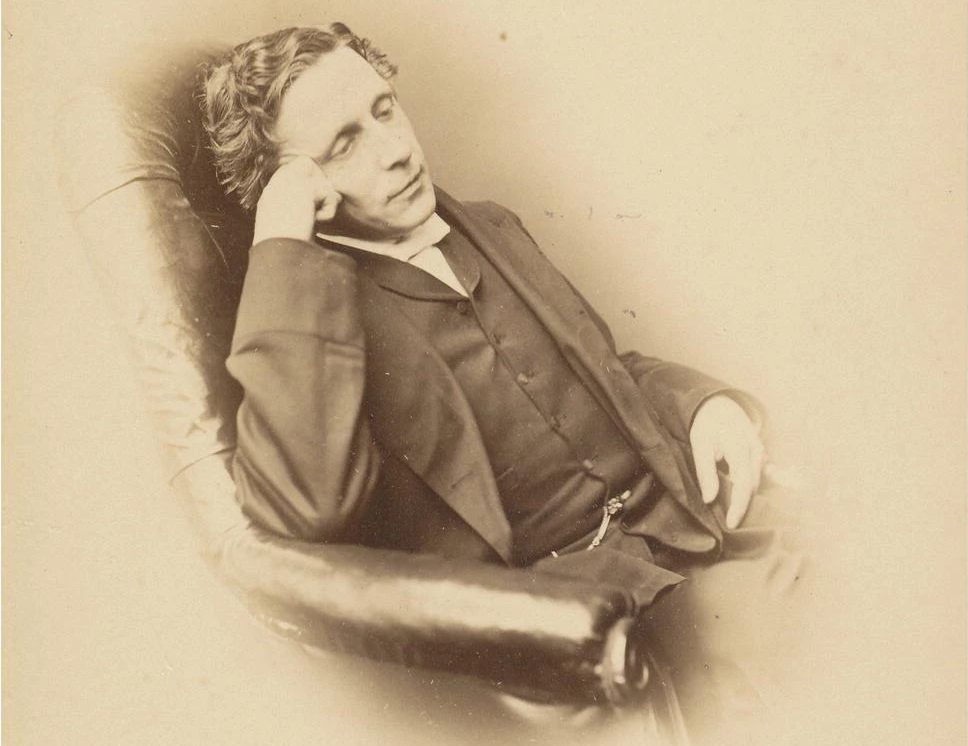
\includegraphics[width= 1\linewidth]{1}
		\vspace*{-15pt}
	\end{figure}
	Như vậy, xuất phát từ những đối tượng mà con người nhìn thấy, hay tưởng tượng ra, người ta gọi chúng là những phần tử, để từ đó tạo nên tập hợp. Mọi thứ con người có thể nhìn thấy đều hữu hạn, nhưng tưởng tượng thì vô hạn. Gần gũi nhất là những con số. Bạn đã bao giờ thử đếm từ một đến một tỷ chưa? Cho dù ngày nay bạn có thể có một tỷ đồng, thậm chí một tỷ đô la, nhưng tôi cá là bạn sẽ không thể đủ sức đếm từ một đến một tỷ. Ấy vậy mà, một tỷ cũng chỉ là một con số hữu hạn, hoàn toàn ``bé nhỏ" trước những ``vô hạn" trong toán học.
	\vskip 0.1cm
	Các nhà toán học luôn đầy tham vọng. Điển hình là việc họ không bao giờ thỏa mãn với một con số cụ thể nào cả. Ngay cả sự vô hạn của các số tự nhiên cũng là quá hạn hẹp đối với họ. Cantor phát hiện ra rằng hóa ra tập các số thực thật sự ``nhiều" hơn tập các số tự nhiên. Thế nào là nhiều hơn đối với những tập vô hạn là một điều không đơn giản. Ta hãy lấy ví dụ để hình dung về sự nhiều hơn một cách có hệ thống.
	\vskip 0.1cm
	Nếu tập $A$ có $2$ phần tử, ví dụ $A=\{0,1\}$, thì $A$ có cả thảy $4$ tập con: rỗng, $\{0\}, \{1\}$ và chính $A$. Tương tự, bạn đọc có thể kiểm tra, nếu $B=\{0,1,2\}$ thì $B$ có cả thảy $8$ tập con. Cantor coi các tập con của $A$, hay của $B$, là những phần tử, chúng tạo nên những tập hợp mới -- tập các tập con, ký hiệu là $P(A)$ hay $P(B)$. Mọi việc khá đơn giản nếu chỉ xét những tập với một số hữu hạn phần tử, nhưng sẽ không còn đơn giản nếu xét tập vô hạn, ví dụ tập các số tự nhiên. Có thể liệt kê, một cách tuần tự tất cả các tập con của tập các số tự nhiên như ta vừa làm với $A$ ở trên hay không? 
	\vskip 0.1cm
	Hóa ra là không thể, Cantor đã \textit{chứng minh} được điều đó. ``Chứng minh được một điều gì là không thể thực hiện được" rõ ràng là không tầm thường phải không các bạn? Cantor đã gây sốc cho cộng đồng toán học với Lý thuyết tập hợp của mình những năm cuối thế kỷ XIX. Không ít nhà toán học phản đối ông kịch liệt.
	\vskip 0.1cm
	Tuy nhiên, không lâu sau đó, lý thuyết tập hợp mà Cantor xây dựng được nhắc đến như là ``lý thuyết tập hợp ngây thơ". Sau khi Cantor ``tháo nút chai", tư duy toán học phát triển mạnh mẽ, người ta phát hiện ra rằng làm việc với những thứ vô hạn hóa ra phức tạp hơn nhiều so với những gì mà Cantor đã ``ngây thơ" hình dung. 
	\vskip 0.1cm
	Ta hãy phát triển ý tưởng trên của Cantor về các tập con. Ta hãy coi mỗi tập hợp như một phần tử và xét tập hợp mà chúng tạo nên. Bản chất của toán học nằm ở sự tự do của nó, Cantor đã dạy thế! Có gì hạn chế được chúng ta tưởng tượng, hay tư duy đâu!
	\vskip 0.1cm
	Chỉ có một bất hợp lý nhỏ được vài nhà toán học để ý. Nếu gọi $X$ là tập tất cả các tập hợp thì hóa ra $X$ lại chứa chính nó như một phần tử! Liệu các bạn có thể hình dung được một tập hợp chứa chính bản thân mình như một phần tử không? Tuy nhiên, việc chúng ta không/chưa hình dung được không có nghĩa là điều đó không tồn tại. 
	\vskip 0.1cm
	Thế nhưng, ta hãy xét tập hợp con $Y$ của $X$ bao gồm các phần tử -- mỗi phần tử bản thân là một tập hợp các bạn nhé -- với tính chất: nó không chứa chính nó như một phần tử. Nói cách khác, một tập hợp $A$ là một phần tử của $Y$ nếu $A$ không chứa $A$ như một phần tử.
	\vskip 0.1cm
	Ví dụ, bản thân $X$ không là phần tử của $Y$, vì $X$ chứa $X$ như một phần tử. 
	\vskip 0.1cm
	Câu hỏi: $Y$ có là phần tử của $Y$ không? 
	\vskip 0.1cm
	Tất nhiên, câu trả lời chỉ có thể là Có hoặc Không.
	\vskip 0.1cm
	Tuy nhiên:
	\vskip 0.1cm
	-- Nếu $Y$ chứa $Y$ như một phần tử, thì theo định nghĩa của $Y$, $Y$ không phải là phần tử của $Y$;
	\vskip 0.1cm
	-- Nếu $Y$ không chứa $Y$ như một phần tử, thì theo định nghĩa của $Y$, $Y$ là phần tử của $Y$!
	\vskip 0.1cm
	Vậy, tự do trong toán học cũng bị hạn chế.
\end{multicols}
